%
%==> Section: TikZ libraries
%
\section{
  Ti$k$Z libraries
}
%
%==> TikZ libraries
%
\begin{frame}
  \frametitle{
    Ti$k$Z libraries
  }
  \begin{itemize}
  \item
    To provide simpler methods to create complex structures
    libraries for Ti$k$Z has \textcolor{purple}{\tt $\backslash$usetikzlibary}
  \item
    Different examples are: \textcolor{blue}{ \tt decorations.fractals},  \textcolor{blue}{ \tt arrows}, \textcolor{blue}{ \tt backgrounds}, \textcolor{blue}{ \tt intersections}, and \textcolor{blue}{ \tt shapes.geometric}.
  \end{itemize}
\end{frame}

%
%==> Examples
%
\begin{frame}[fragile]
  \frametitle{
    And now for some examples
  }

  First you must add

  \begin{lstlisting}
    \usetikzlibrary{backgrounds}
  \end{lstlisting}
  
  to your preamble

  \begin{center}
    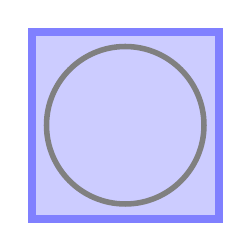
\begin{tikzpicture}
  [background rectangle/.style={fill=blue!20,
      draw=blue!50,line width=3pt},
    show background rectangle]
  \draw[line width=2pt,color=gray]
  (2,2) circle[radius=1];
\end{tikzpicture}

  \end{center}

  \lstinputlisting{./tex/src/tikz_lib_backgrounds_example.tex}

\end{frame}

%
%==> Koch snowflake
%
\begin{frame}[fragile]
  \begin{itemize}
  \item
    For the Koch snowflake, first you must add

    \begin{lstlisting}
      \usetikzlibrary{decorations.fractals}
    \end{lstlisting}

    to your preamble

    % Generate image
    \begin{center}
      
\begin{tikzpicture}[decoration=Koch
          snowflake,draw=blue,fill=green!20,thick]
        \filldraw decorate{ decorate{ (0,0) --
            ++(60:1) -- ++(-60:1) -- cycle}};
      \end{tikzpicture}
    \end{center}
    
    % Source file
    \begin{lstlisting}
      
\begin{tikzpicture}[decoration=Koch
          snowflake,draw=blue,fill=green!20,thick]
        \filldraw decorate{ decorate{ (0,0) --
            ++(60:1) -- ++(-60:1) -- cycle}};
      \end{tikzpicture}
    \end{lstlisting}

  \item
    Don't forget to put the correct Ti$k$Z library in your preamble.
    
  \end{itemize}

\end{frame}
